\newpage
\lecture{6}{Применения сингулярного разложения.}

\subsection{Псевдорешения СЛУ.}

Рассмотрим систему линейных алгебраических уравнений:
\[
    Ax=b,\quad A\in\Cx^{m\times n},\quad b\in\Cx^{n},\quad x=\text{?}    
\]

Иногда бывает так, что система не имеет решения, но очень хочется что-то предъявить в качестве решения. Тогда вводят понятие обобщенного 
решения. Для этого используется некоторая векторная норма.

\begin{definition}
    Вектор вида $r(x)=b-Ax$ называется \mdef{невязкой} вектора $x$ для системы $Ax=b$.
\end{definition}

Соответственно можем поставить задачу минимизации невязки для некоторой векторной нормы:
\[
    \min_{x}\|r(x)\| = \text{?}
\]
Мы возьмем в качестве нормы возьмем евклидову:
\[
    \|x\|=\|x\|_2=\sqrt{\sum_{i=1}^n |x_i|^2}.
\]
\begin{definition}
    Любой вектор, минимизирующий длину невязки, называется \mdef{псевдорешением}.
\end{definition}

Опишем множество всех псевдорешений. Подумаем геометрически над задачей. Пусть имеется $\im(A)$ (напомним, что $\im(A)=\{y:\ \exists x,\, Ax=y\}$) и произвольный 
вектор $b$ (смотри рисунок \ref{fig:im}).

\begin{figure}[!ht]
    \centering
    

\tikzset{every picture/.style={line width=0.75pt}} %set default line width to 0.75pt        

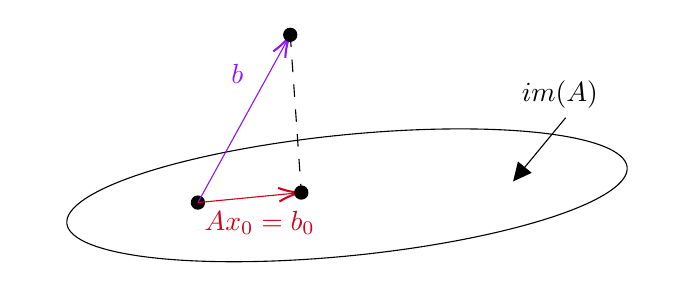
\begin{tikzpicture}[x=0.75pt,y=0.75pt,yscale=-1,xscale=1]
%uncomment if require: \path (0,300); %set diagram left start at 0, and has height of 300

%Shape: Ellipse [id:dp7555518550305362] 
\draw   (22.21,101.67) .. controls (52.33,83.99) and (132.02,69.67) .. (200.21,69.67) .. controls (268.39,69.67) and (299.25,83.99) .. (269.13,101.67) .. controls (239,119.34) and (159.31,133.67) .. (91.13,133.67) .. controls (22.94,133.67) and (-7.91,119.34) .. (22.21,101.67) -- cycle ;
%Straight Lines [id:da8611871472064767] 
\draw    (251,64.33) -- (227.58,92.69) ;
\draw [shift={(225.67,95)}, rotate = 309.56] [fill={rgb, 255:red, 0; green, 0; blue, 0 }  ][line width=0.08]  [draw opacity=0] (8.93,-4.29) -- (0,0) -- (8.93,4.29) -- cycle    ;
%Flowchart: Connector [id:dp3708456265538911] 
\draw  [fill={rgb, 255:red, 0; green, 0; blue, 0 }  ,fill opacity=1 ] (70.67,105.17) .. controls (70.67,103.42) and (72.08,102) .. (73.83,102) .. controls (75.58,102) and (77,103.42) .. (77,105.17) .. controls (77,106.92) and (75.58,108.33) .. (73.83,108.33) .. controls (72.08,108.33) and (70.67,106.92) .. (70.67,105.17) -- cycle ;
%Straight Lines [id:da7865576084467163] 
\draw [color={rgb, 255:red, 144; green, 19; blue, 254 }  ,draw opacity=1 ]   (73.83,105.17) -- (117.37,26.09) ;
\draw [shift={(118.33,24.33)}, rotate = 478.83] [color={rgb, 255:red, 144; green, 19; blue, 254 }  ,draw opacity=1 ][line width=0.75]    (10.93,-3.29) .. controls (6.95,-1.4) and (3.31,-0.3) .. (0,0) .. controls (3.31,0.3) and (6.95,1.4) .. (10.93,3.29)   ;
%Flowchart: Connector [id:dp6219908990509146] 
\draw  [fill={rgb, 255:red, 0; green, 0; blue, 0 }  ,fill opacity=1 ] (115.17,24.33) .. controls (115.17,22.58) and (116.58,21.17) .. (118.33,21.17) .. controls (120.08,21.17) and (121.5,22.58) .. (121.5,24.33) .. controls (121.5,26.08) and (120.08,27.5) .. (118.33,27.5) .. controls (116.58,27.5) and (115.17,26.08) .. (115.17,24.33) -- cycle ;
%Straight Lines [id:da6955868213451586] 
\draw  [dash pattern={on 4.5pt off 4.5pt}]  (118.33,24.33) -- (123.67,100.33) ;
%Straight Lines [id:da6164220853373175] 
\draw [color={rgb, 255:red, 208; green, 2; blue, 27 }  ,draw opacity=1 ]   (73.83,105.17) -- (121.68,100.53) ;
\draw [shift={(123.67,100.33)}, rotate = 534.46] [color={rgb, 255:red, 208; green, 2; blue, 27 }  ,draw opacity=1 ][line width=0.75]    (10.93,-3.29) .. controls (6.95,-1.4) and (3.31,-0.3) .. (0,0) .. controls (3.31,0.3) and (6.95,1.4) .. (10.93,3.29)   ;
%Flowchart: Connector [id:dp6806386155739477] 
\draw  [fill={rgb, 255:red, 0; green, 0; blue, 0 }  ,fill opacity=1 ] (120.5,100.33) .. controls (120.5,98.58) and (121.92,97.17) .. (123.67,97.17) .. controls (125.42,97.17) and (126.83,98.58) .. (126.83,100.33) .. controls (126.83,102.08) and (125.42,103.5) .. (123.67,103.5) .. controls (121.92,103.5) and (120.5,102.08) .. (120.5,100.33) -- cycle ;

% Text Node
\draw (228.67,45) node [anchor=north west][inner sep=0.75pt]   [align=left] {$\displaystyle \operatorname{im}( A)$};
% Text Node
\draw (88.67,37.33) node [anchor=north west][inner sep=0.75pt]  [color={rgb, 255:red, 144; green, 19; blue, 254 }  ,opacity=1 ] [align=left] {$\displaystyle b$};
% Text Node
\draw (75.83,108.17) node [anchor=north west][inner sep=0.75pt]  [color={rgb, 255:red, 208; green, 2; blue, 27 }  ,opacity=1 ] [align=left] {$\displaystyle Ax_{0} =b_{0}$};


\end{tikzpicture}

    \caption{К задаче о поиске псевдорешений.}
    \label{fig:im}
\end{figure}

Понятно, что для минимизации нормы, нужно опустить перпендикуляр на множество $\im(A)$, тогда для соответствующего 
вектора (на рисунке $Ax_0=b_0$) система $Ax=b_0$ уже будет совместной.

Итак, множество всех псевдорешений есть множество всех решений совместной системы $Ax=b_0\ (=Ax_0)$.

Обычно есть желание найти какой-нибудь один вектор в качестве псевдорешения, то есть нужен некоторый критерий отбора вектора среди всех векторов,
минимизирующих длину невязки. В качестве такого критерия часто берут длину вектора, то есть среди всех таких векторов ищут минимальный по длине.

\begin{definition}
    Псевдорешение минимальной длины называется \mdef{нормальным} псевдорешение.
\end{definition}

Итак, более формально, имеем множество решений системы $Ax=b_0\ (=Ax_0)$, то есть $x = x_0+\ker(A)$ (напомним, что $\ker(A)=\{x:\ Ax=0\}$).
Рассуждая снова геометрически (смотри рисунок \ref{fig:ker}), получим, что искомое нормальное псевдорешение $z\bot \ker(A)$.

\begin{figure}[!ht]
    \centering
    

\tikzset{every picture/.style={line width=0.75pt}} %set default line width to 0.75pt        

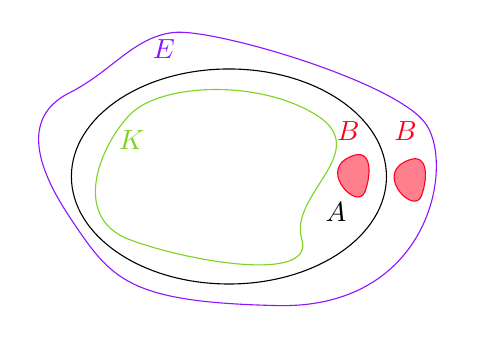
\begin{tikzpicture}[x=0.75pt,y=0.75pt,yscale=-1,xscale=1]
%uncomment if require: \path (0,300); %set diagram left start at 0, and has height of 300

%Shape: Ellipse [id:dp21713989696743696] 
\draw   (40,120.8) .. controls (40,92.19) and (73.98,69) .. (115.9,69) .. controls (157.82,69) and (191.8,92.19) .. (191.8,120.8) .. controls (191.8,149.41) and (157.82,172.6) .. (115.9,172.6) .. controls (73.98,172.6) and (40,149.41) .. (40,120.8) -- cycle ;
%Shape: Polygon Curved [id:ds9621936473500847] 
\draw  [color={rgb, 255:red, 126; green, 211; blue, 33 }  ,draw opacity=1 ] (68,91.2) .. controls (82.6,75.8) and (130.2,73.8) .. (158,91.2) .. controls (185.8,108.6) and (144.4,129.6) .. (151,151) .. controls (157.6,172.4) and (96.2,161.8) .. (68,151.2) .. controls (39.8,140.6) and (53.4,106.6) .. (68,91.2) -- cycle ;
%Shape: Polygon Curved [id:ds46698398853897394] 
\draw  [color={rgb, 255:red, 144; green, 19; blue, 254 }  ,draw opacity=1 ] (39.2,80.4) .. controls (59.2,70.4) and (70.08,53.43) .. (89.4,51.4) .. controls (108.72,49.37) and (197.4,75.4) .. (211,95.8) .. controls (224.6,116.2) and (212.2,184.6) .. (139.4,183) .. controls (66.6,181.4) and (59.2,170.4) .. (39.2,140.4) .. controls (19.2,110.4) and (19.2,90.4) .. (39.2,80.4) -- cycle ;
%Shape: Polygon Curved [id:ds1249511800221168] 
\draw  [color={rgb, 255:red, 255; green, 0; blue, 31 }  ,draw opacity=1 ][fill={rgb, 255:red, 255; green, 0; blue, 31 }  ,fill opacity=0.5 ] (199.8,114.2) .. controls (212.2,107) and (212,121.2) .. (208.6,130.2) .. controls (205.2,139.2) and (187.4,121.4) .. (199.8,114.2) -- cycle ;
%Shape: Polygon Curved [id:ds831095716110374] 
\draw  [color={rgb, 255:red, 255; green, 0; blue, 31 }  ,draw opacity=1 ][fill={rgb, 255:red, 255; green, 0; blue, 31 }  ,fill opacity=0.5 ] (172.6,112.2) .. controls (185,105) and (184.8,119.2) .. (181.4,128.2) .. controls (178,137.2) and (160.2,119.4) .. (172.6,112.2) -- cycle ;

% Text Node
\draw (161.2,132.2) node [anchor=north west][inner sep=0.75pt]   [align=left] {$\displaystyle A$};
% Text Node
\draw (61.6,97.2) node [anchor=north west][inner sep=0.75pt]   [align=left] {$\displaystyle \textcolor[rgb]{0.49,0.83,0.13}{K}$};
% Text Node
\draw (78,53.8) node [anchor=north west][inner sep=0.75pt]   [align=left] {$\displaystyle \textcolor[rgb]{0.56,0.07,1}{E}$};
% Text Node
\draw (166.8,93) node [anchor=north west][inner sep=0.75pt]   [align=left] {$\displaystyle \textcolor[rgb]{1,0,0.13}{B}$};
% Text Node
\draw (194.4,93) node [anchor=north west][inner sep=0.75pt]   [align=left] {$\displaystyle \textcolor[rgb]{1,0,0.13}{B}$};


\end{tikzpicture}

    \caption{Нормальное псевдорешение.}
    \label{fig:ker}
\end{figure}

Суммируя сказанное можно сформулировать утверждение:
\begin{claim}
    \label{lect6:cl:1}
    Нормальное псевдорешение $z$ системы $Ax=b$ однозначно определяется двумя условиями:
    \begin{enumerate}[label=(\arabic*)]
        \item $b-Az\bot \im(A)$,
        \item $z\bot \ker(A)$.
    \end{enumerate}
\end{claim}

\begin{task}
    Доказать, что система $A^*Ax=A^*b$ всегда совместна и множество ее решений совпадает с множеством псевдорешений системы $Ax=b$.
\end{task}

\subsection{Формула для нормального псевдорешения.}

Рассмотрим сингулярное разложение матрицы (ранг матрицы равен $r$):
\[
    A=\sum_{i=1}^r \sigma_i\vect{v}_i\vect{u}_i^*.
\]
Далее имеем $\vect{v}_1,\,\ldots\,\, \vect{v}_m$~--- ортонормированный базис пространства $\Cx^m$, то есть 
\[
    \vect{b} = \sum_{i=1}^m b_i\vect{v}_i\Rightarrow (\vect{v}_i,\, \vect{b})=\vect{v}_i^*\vect{b}=b_i\Rightarrow \vect{b}=\sum_{i=1}^m(\vect{v}_i^*\vect{b})\vect{v}_i.
\]

\begin{claim}
    Нормальное псевдорешение $z$ имеет вид  
    \[
        \vect{z} = \sum_{i=1}^r \dfrac{\vect{v}_i^*\vect{b}}{\sigma_i}\vect{u}_i.    
    \]

    \begin{proof}
        
        Для доказательства достаточно проверить оба условия из утверждения \ref{lect6:cl:1}. 
        \begin{enumerate}[label=(\arabic*)]
            \item Для начала заметим, что $\im(A)=L(\vect{v}_1,\,\ldots,\,\vect{v}_r)$. Рассмотрим вектор $\vect{b}-A\vect{z}$:
            \[
                \vect{b}-A\vect{z}=\underbrace{\sum_{i=1}^r \left(\vect{v}^*_i\vect{b}-\dfrac{\vect{v}_i^*\vect{b}}{\sigma_i}\sigma_i\right)\vect{v}_i}_0
                +\sum_{i=r+1}^m \left(\vect{v}_i^*\vect{b}\right)\vect{v}_i.
            \]
            То есть вектор $\vect{b}-A\vect{z}\in L(\vect{v}_{r+1},\,\ldots,\, \vect{v}_m)$. Значит условие (1) выполняется.
            \item Аналогично, $z\in L(\vect{u}_1,\,\ldots,\, \vect{u}_r)$, $\ker(A)=L(\vect{u}_{r+1},\,\ldots,\, \vect{u}_n)$. 
        \end{enumerate}

    \end{proof}
\end{claim}

\begin{exercise}
    Рассмотрим систему $0\cdot x = 1$. Данная система не имеет решений, но она имеет нормальное псевдорешение. Длина невязки в данном случае равна 1 вне зависимости от вектора 
    $x$. Значит минимальный по длине вектор~--- нулевой. Итак, $z(0)=0$.

    Немного видоизменим систему: $\varepsilon\cdot x(\varepsilon) = 1$. 
    Понятно, что теперь $z(\varepsilon)=\dfrac{1}{\varepsilon}$. Но тогда 
    \[
        z(\varepsilon) - z(0)=\dfrac{1}{\varepsilon}\xrightarrow[\varepsilon\to 0]{}\infty.
    \]
    Полученный результат указывает на проблему: в самом деле, если чуть-чуть изменить значения матрицы, нормальные псевдорешения меняются кардинальным образом.
\end{exercise}

\subsection{Поиск нормальных псевдорешений.}
Допустим теперь, что нужно найти нормальное псевдорешение для системы, которая неизвестна, 
но известны приближения: $A_{\varepsilon}\approx A$ и $\vect{b}_{\varepsilon}\approx \vect{b}$, то есть 
$\|A_{\varepsilon}-A\|\leqslant \varepsilon$ и $\|\vect{v}_{\varepsilon}-\vect{b}\|\leqslant \varepsilon$.
Для решения данной задачи предлагается метод регуляризации.

\subsubsection{Метод регуляризации.}
Возьмем некоторое $\alpha>0$. Рассмотрим систему:
\[
    (A^*_{\varepsilon}A_{\varepsilon}+\alpha I)\vect{z}_{\varepsilon,\alpha}=A_{\varepsilon}^{*}\vect{b}.    
\]
Данная система имеет единственное решение для любого $\alpha>0$, в самом деле матрица $A^*_{\varepsilon}A_{\varepsilon}$~--- эрмитова неотрицательно 
определенная (смотри определение ниже) матрица. 

\begin{definition}
    Матрица $H$ называется \mdef{неотрицательно определенной}, если $(H\vect{x},\, \vect{x})\geqslant 0\ \forall\vect{x}$.
\end{definition}

\begin{definition}
    Матрица $H$ называется \mdef{положительно определенной}, если $(H\vect{x},\, \vect{x})> 0\ \forall\vect{x}$.
\end{definition}

Тогда матрица $A^*_{\varepsilon}A_{\varepsilon}+\alpha I$ является положительно определенной эрмитовой матрицей. 
Предлагается взять в качестве приближения к нормальному псевдорешению исходной системы решение новой системы.
Пусть $\vect{z}_0$~--- нормальное псевдорешение исходной системы. Тогда справедлива следующая теорема.

\begin{theorem}
    $\|\vect{z}_{\varepsilon,\, \sqrt{\varepsilon}}-\vect{z}_0\|=O(\sqrt{\varepsilon})\to 0$ при $\varepsilon\to 0$.
    
    \begin{proof}
        
        Итак, $A_0=A$. Рассмотрим систему $(A^*A+\alpha I)\vect{z}_{0,\, \alpha}=A^*\vect{b}$.
        Докажем, что $\|\vect{z}_{0,\,\alpha}-\vect{z}_0\|=O(\alpha)$. Вспомним формулу для нормального псевдорешения:
        \[
            \vect{z}_0=\sum_{i=1}^r\dfrac{\vect{v}_i^*\vect{b}}{\sigma_i}\vect{u}_i.\quad \vect{z}_{0,\,\alpha}=
            \sum_{i=1}^r\dfrac{\sigma_i}{\sigma_i^2+\alpha}(\vect{v}_i^*\vect{b})\vect{u}_i.
        \]
        В самом деле распишем обе стороны:
        \begin{align*}
            &A^*A+\alpha I=\sum_{i=1}^r(\sigma_i^2+\alpha)\vect{u}_i\vect{u}_i^*+\sum_{i=r+1}^n \alpha\vect{u}_i\vect{u}_i^*\\
            &A^*\vect{b}=\sum_{i=1}^r \sigma_i(\vect{v}_i^*\vect{b})\vect{u}_i.
        \end{align*}

        Оценим теперь разность: 
        \[
            \vect{z}_0-\vect{z}_{0,\,\alpha}=\sum_{i=1}^r\dfrac{\alpha}{\sigma_i(\sigma_i^2+\alpha)}(\vect{v}_i^*\vect{b})\vect{u}_i.
        \]

        Теперь рассмотрим $\vect{z}_{0,\,\alpha}-\vect{z}_{\varepsilon,\, \alpha}$. Умножим на матрицу $A^*_{\varepsilon}A_{\varepsilon}+\alpha I$:
        \[
            (A^*_{\varepsilon}A_{\varepsilon}+\alpha I)(\vect{z}_{0,\,\alpha}-\vect{z}_{\varepsilon,\, \alpha})=((A^*_{\varepsilon}A_{\varepsilon}+\alpha I) -
            (A^*A+\alpha I))\vect{z}_{0,\,\alpha}+\underbrace{(A^*A+\alpha I)\vect{z}_{0,\,\alpha}}_{A^*\vect{b}}-
            \underbrace{(A^*_{\varepsilon}A_{\varepsilon}+\alpha I)\vect{z}_{\varepsilon,\,\alpha}}_{A_{\varepsilon}^*\vect{b}_{\varepsilon}}.
        \]
        Тогда имеем 
        \[
            \vect{z}_{0,\,\alpha}-\vect{z}_{\varepsilon,\,\alpha}=(A^*_{\varepsilon}A_{\varepsilon}+\alpha I)^{-1}((A^*_{\varepsilon}A_{\varepsilon}-A^*A)\vect{z}_{0,\,\alpha}+
            A^*\vect{b}-A_{\varepsilon}^*\vect{b}_{\varepsilon}^*).
        \]
        Следовательно,
        \begin{align*}
            \|\vect{z}_{0,\,\alpha}-\vect{z}_{\varepsilon,\,\alpha}\|&\leqslant \dfrac{1}{\alpha}\left(\|A^*_{\varepsilon}(A_{\varepsilon}-A)+(A^*_{\varepsilon}-A^*)A\|
            \cdot\|\vect{z}_{0,\,\alpha}\|+\|A^*(\vect{b}-\vect{b}_{\varepsilon}+(A^*-A_{\varepsilon}^*)\vect{b}_{\varepsilon}\|\right)\\
            &\leqslant\dfrac{1}{\alpha}\left(((\|A\|+\varepsilon)\varepsilon+\|A\|\varepsilon)(\|\vect{z}_0\|+c\alpha)+\|A\|\varepsilon+(\|\vect{b}\|+\varepsilon)\varepsilon\right)
            \leqslant\dfrac{c_0\varepsilon}{\alpha}. 
        \end{align*}
        И окончательно,
        \[
            \|\vect{z}_{\varepsilon,\,\alpha}-\vect{z}_0\|\leqslant \dfrac{c_0\varepsilon}{\alpha}+c\alpha=[\alpha = \sqrt{\varepsilon}]=(c_0+c)\sqrt{\varepsilon}.    
        \]
    \end{proof} 
\end{theorem}